\documentclass[10pt,twocolumn,letterpaper]{article}
\ifdefined\reviewcopy
\usepackage[review]{cvpr}
\else
\usepackage[pagenumbers]{cvpr}
\fi
\usepackage{microtype}
\usepackage[pagebackref,breaklinks,colorlinks,allcolors=blue]{hyperref}
\def\paperID{0000}
\def\confName{CVPR}
\def\confYear{2026}
\newcommand{\EpisodeCount}{145}
\newcommand{\ProbeCount}{739}
\newcommand{\PairCount}{98}
\newcommand{\SourceCount}{11}
\newcommand{\ProfileCount}{20}
\newcommand{\OracleCount}{70}
\newcommand{\ProductCount}{4,053,285}
\newcommand{\EdgeCount}{39,989,367}
\newcommand{\MaxGap}{18}
\newcommand{\OldLabels}{1,802,728}

\title{BrickPlan: Diagnosing Future Action Cost and Error Recovery\\in Visual Assembly Planning}
\author{Benchmark research release 2.1\\Population model and human studies pending}
\begin{document}
\maketitle

\begin{abstract}
Visual assembly planning requires predicting how an action changes later
access, workspace occupancy, and unfinished work. Final-shape accuracy and
solution length alone do not isolate these abilities. We introduce
BrickPlan, an executable benchmark with exact future-cost and recovery
labels under a declared, finite assembly abstraction. Original LDraw
geometry determines qualified motions and connectivity; a limited rack
and persistent off-assembly inspection ledger couple decisions over time.
The release contains \EpisodeCount{} interactive episodes and
\ProbeCount{} diagnostic questions from \SourceCount{} source groups.
Matched sequence pairs balance early and late conflicts, geometry
contrasts change future legality while preserving registered pieces and
plans, and delayed-repair questions exclude the terminal goal from
recovery credit. We release native-resolution observations, a categorized
question explorer, exact evaluators, and a real four-call local VLM trace.
Structural controls reveal both scope and limits: closure greedy completes
384 of 435 task-runs but only 266 optimally, while full closure A* solves
every run with at most 4,372 expansions. A five-step prefix shortcut scores
66.7\% on the sequence tests. These results validate measurable scheduling
and diagnostic distinctions, not necessary internal reasoning depth.
Population VLM and human results remain unmeasured.
\end{abstract}

\section{Introduction}
An assembly action can be legal now and expensive later. Removing a part
may consume the last available holder before a deeper part is accessible;
reattaching another part may block unfinished work. If a planner notices
an error only after several more operations, undoing its latest action
need not restore an efficient completion. Measuring these effects requires
more than recognizing brick types or comparing a final image.

BrickPlan asks a specific question: can a visual agent predict the
\emph{future action cost} of a decision, and recover after that decision
has propagated? We separate three observable failures: an immediately
rejected operation, a legal action that increases exact remaining cost,
and a later failure to return to an optimal completion corridor.
The geometry and tasks are small enough to label these distinctions
exhaustively. This deliberate restriction enables exact diagnostics
at the expense of unrestricted manipulation.

A motivating audit illustrates why such care is necessary. For a preceding
assembly-only bank, an occupied-blocker closure formula reproduced all
\OldLabels{} stored state--goal costs. Long solutions in that bank did
not establish deep planning. Our task adds limited external storage and
inspection work that persists after reattachment. Static geometric
relations remain useful, but physical occupancy alone no longer specifies
the mission state or its exact cost.

We make three contributions. First, we define a visual assembly task with
certified, state-dependent resource and work obligations, accompanied by
both interactive episodes and explicit diagnostic question formats.
Second, we construct sequence, geometry, appearance, and delayed-repair
controls that expose particular shortcuts and confounds. Third, we release
the observation, execution, scoring, and publication pipeline together,
including exact software controls and an authenticated model integration
case. We distinguish these contributions from empirical claims that await
a larger model and human study.

\begin{figure*}[t]
\centering
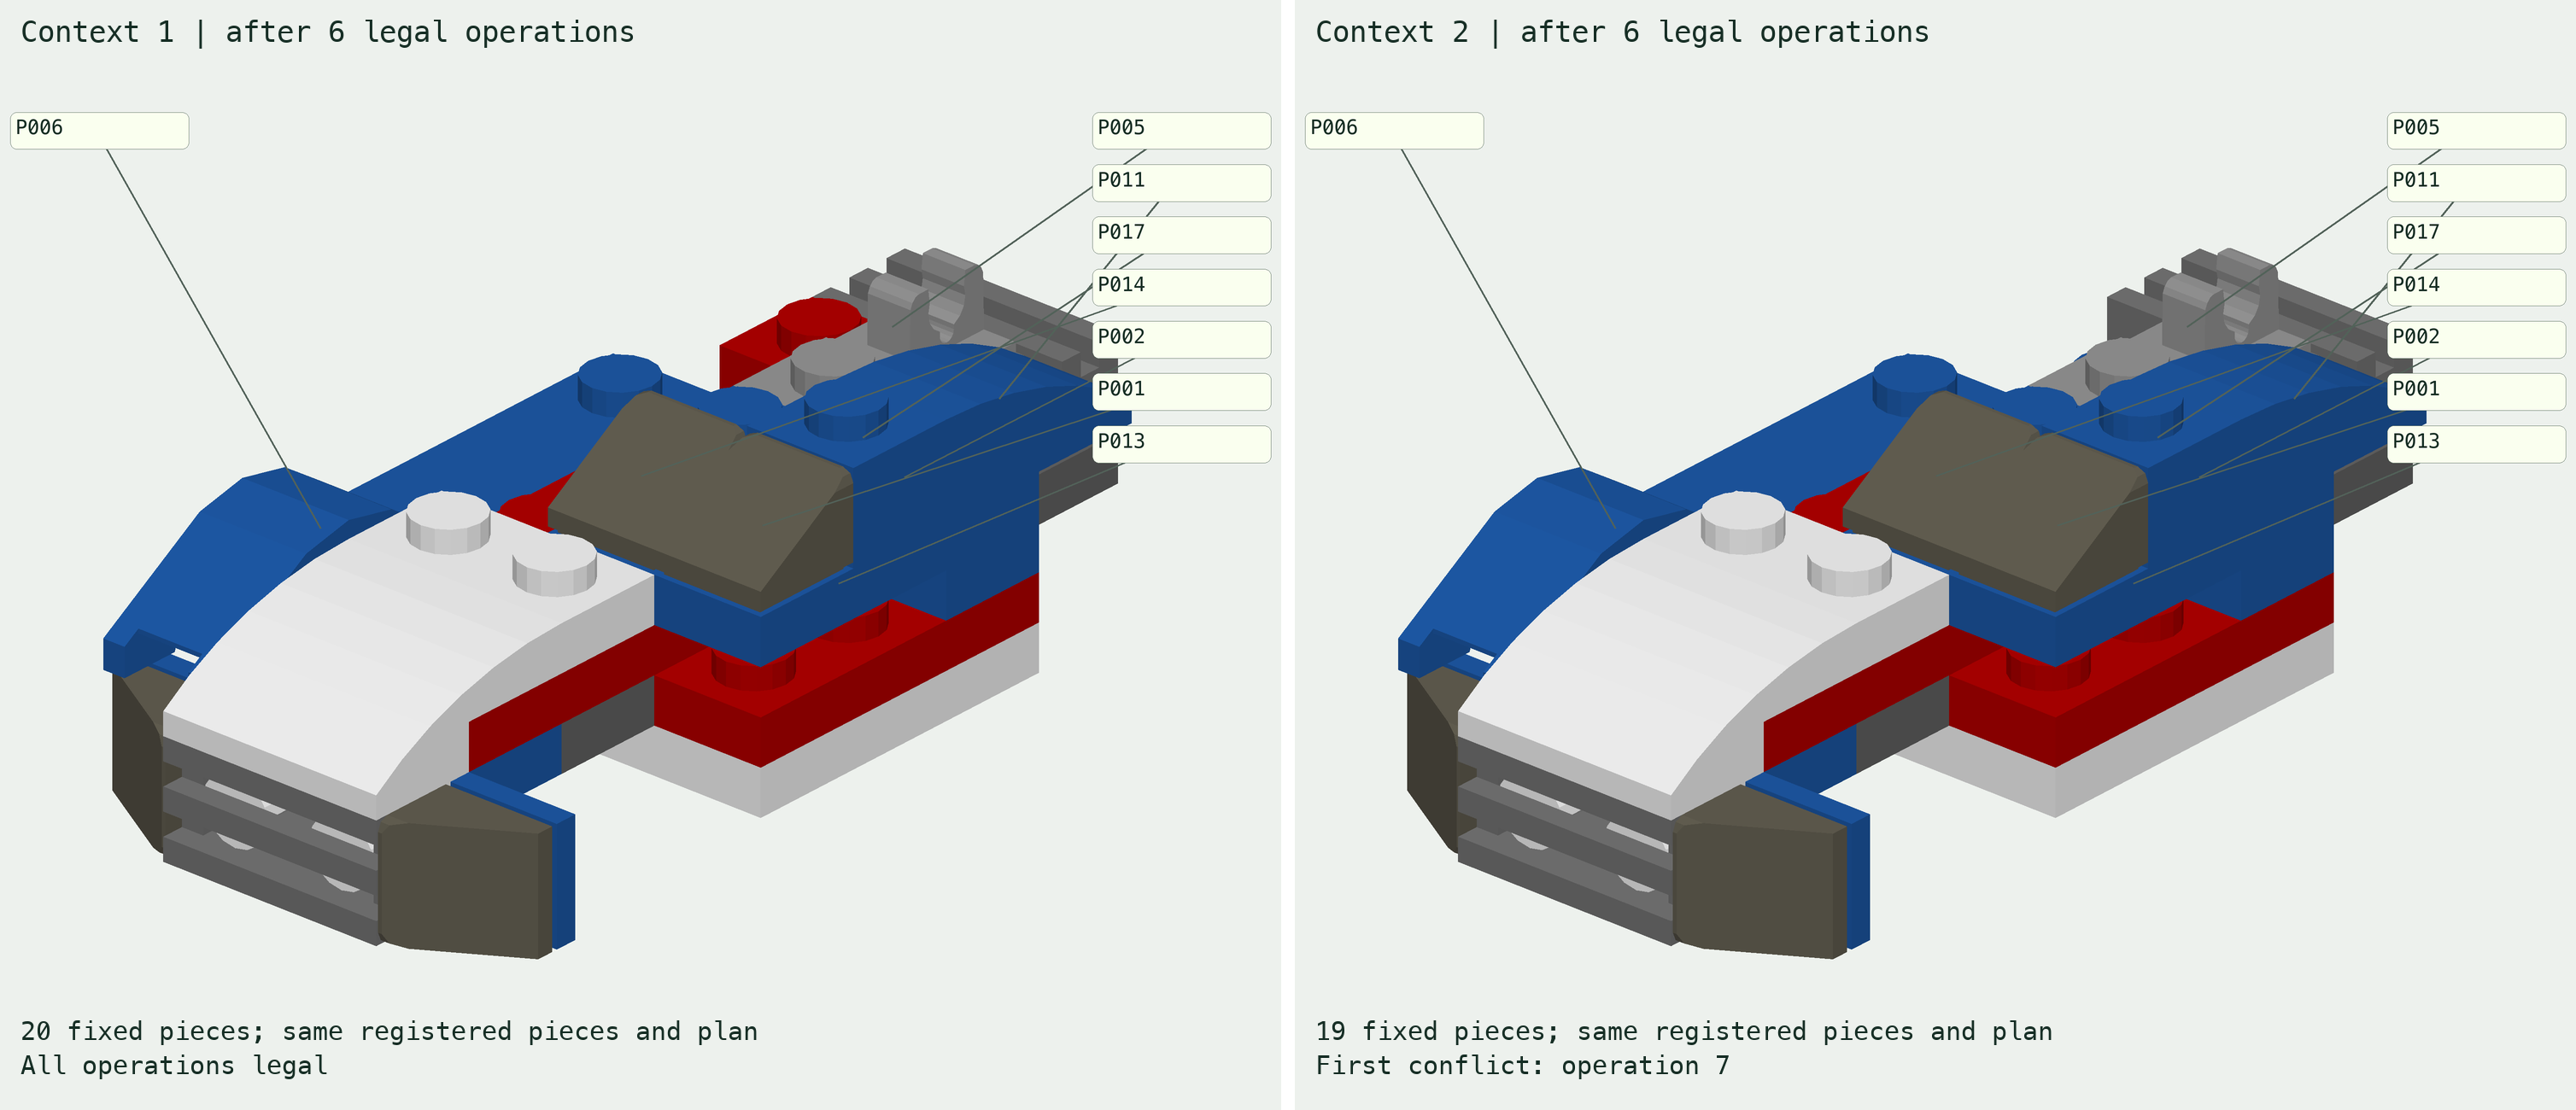
\includegraphics[width=.95\textwidth]{figures/geometry-contrast.png}
\caption{An actual answer-changing geometry pair after its shared
six-operation legal prefix. Registered pieces, original poses, initial
occupancy, goal, rack, work orders, and proposed plan are matched. The
fixed context differs by one original source piece. Context 1 permits the
whole sequence; context 2 rejects operation 7. These are qualified induced
source assemblies, not edited relation labels. The unequal fixed-part
counts remain a confound.}
\label{fig:geometry}
\end{figure*}

\section{Evaluation design}
\label{sec:design}
\begin{table}[t]
\centering\small
\caption{Experimental conditions. ``Pending'' means no population result
has been collected; the local trace is a single integration case. Model
snapshots and provider settings must be fixed before the study.}
\begin{tabular}{p{.60\columnwidth}p{.29\columnwidth}}
\toprule Condition & Evidence status\\\midrule
Structural policies and exact search & Measured\\
SmolVLM-256M, image input & One failed case\\
Open VLMs, image / structured & Pending\\
Proprietary VLMs, image / structured & Pending\\
Humans, image + registered IDs & Pending\\
Stepwise / explicit-plan prompting & Pending\\
\bottomrule
\end{tabular}
\label{tab:design}
\end{table}

Table~\ref{tab:design} fixes the reporting structure before empirical
collection. Primary outcomes are assigned-episode completion, optimal
completion, and excess operations among successes. Diagnostic accuracies
are reported by question family; pair scores require both members to be
correct. Invalid responses and missing assignments remain visible in
denominators. Software controls with exact relations are separated from
the public image and structured conditions.

The proposed study compares matched source groups and identity seeds
under equal action and observation budgets. For each VLM, both input
conditions use the same executor and answer syntax. A format/cost pilot
should precede the full study, with pilot results retained and identified.
Report model snapshot, provider, prompt, image preprocessing, context
policy, decoding, token usage, and calls per assignment. Human collection
requires recorded instructions, training exposure, participant counts,
and consent procedures before recruitment. No such cohort is claimed here.

Repeated identity seeds and paired questions are correlated observations.
Report per-source results and coverage before a pooled mean. With only
three newly sampled source groups, uncertainty for transfer is necessarily
limited; a large number of questions does not create a large number of
independent assemblies. Stratify errors into parsing, immediate legality,
future cost, diagnosis, and repair so a format failure is not interpreted
as evidence of deep planning failure.

\section{Related work}
LTRON's Break and Make evaluates interactive structural understanding
through disassembly and reconstruction~\cite{ltron}. InstructioNet studies
construction supported by an agent's own explicit visual
instructions~\cite{instructionet}. These establish interactive brick
construction and long sequences; BrickPlan does not claim either as new.
Its narrower registered-site action space permits exact counterfactual
completion costs and event-level recovery labels.

LEGO-Puzzles organizes spatial understanding and sequential reasoning
into explicit task families~\cite{lego}. Its revised version includes
both elementary VQA and a Planning set; it should not be reduced to a
static recognition benchmark. PhyBlock combines hierarchical assembly
and physical-understanding questions~\cite{phyblock}.
Brick-Composer introduces BC-Bench for diverse brick selection and
pose estimation, and trains models with construction and feedback
signals~\cite{composer}. BrickPlan instead fixes legal placement sites
and asks about resource coupling, future legality, and delayed recovery.
It complements these broader spatial tasks rather than replacing them.

Shortest-path search and admissible heuristics are established planning
tools~\cite{astar}. A failed weak policy does not establish computational
hardness. We therefore report a strong static relaxation, resource-aware
dispatch, bounded and full A*, and optimistic shallow-choice bounds.
The research contribution is an audited visual diagnostic instrument;
finite racks or A* are not algorithmic novelties.

\section{Task and observation contract}
\subsection{State, geometry, and actions}
Let $A\subseteq V$ be occupied registered sites, $G\subseteq V$ the
target, $J\subseteq V$ the required inspection sites, and $D\subseteq J$
the completed inspections. The mission state is $x=(A,D)$.
Each physical piece $P_i$ is registered to exactly one original site
$S_i$. Detached pieces occupy universal oversized rack holders:
\begin{equation}
  r(x)=|V\setminus A|\leq K,
\end{equation}
where $K$ is the declared capacity. An \texttt{audit} completes one
pending job only when its piece is detached; completion persists after
reattachment. The terminal physical condition is $A=G,\ D=J$.

An \texttt{attach} or \texttt{detach} must satisfy source-qualified
straight translation, collision, stud-connectivity, registration, and
capacity rules. Fixed pieces form a connected clamped assembly.
All executable positions are original LDraw poses. Qualification uses
guarded inset meshes and prescribed paths; it is not force, gravity,
clutch, hand-access, or arbitrary rigid-body simulation.
The rack is an explicit resource abstraction, not simulated transfer
geometry. Exploded displays are marked reference diagrams and never
executable states.

Each accepted physical operation or audit costs one operation, as does
each rejected operation attempt. Valid camera acquisition and diagnosis
consume their separate budgets; \texttt{finish} explicitly terminates a
completed task. There are 12 additional views and 12 diagnoses per episode.
The action budget is fixed in the released task record before collection.
Source size, work orders, budget, and rack capacity are public constraints.

\subsection{Matched observation conditions}
The image condition provides five PNG panels: current assembly, target,
all-site reference, registered-piece catalog, and rack. Main views are
rendered at $3840\times2880$ and antialiased to $1920\times1440$; individual
catalog pieces have $480\times360$ native tiles. Public P/S registration
and the inspection ledger are textual. Image input omits pose matrices,
installed-site flags, legal-action lists, relation graphs, and exact costs.
These omissions preserve a visual inference component, while explicit
registration and rack inventory simplify correspondence.

The structured condition adds original matrices, part identifiers,
colors, path directions and lengths, and site occupancy. It still omits
the private blocker/support graph. Structural software controls receive
that graph and are a separate privileged condition. Additional acquired
views persist as revision-specific observations. Free 3D orbit and
explosion are available in the unscored practice workbench, outside study
and model observations. Human and model policies share the controlled
observation and submission protocol.

\begin{table*}[t]
\centering\small
\caption{Seven question families in the public explorer. Each question
has a stable ID, complete prompt, state, constraints, answer format, and
scoring rule. Episode families are mutually exclusive presentation groups.}
\begin{tabular}{p{.19\textwidth}p{.38\textwidth}p{.33\textwidth}}
\toprule Family & Question & Response and measurement\\\midrule
Assembly / reconfiguration & Transform the current assembly into the target. & Action sequence; completion and excess cost\\
Finite-resource scheduling & Which operations free the holders needed for later work? & Action sequence under a capacity bound\\
Inspection / persistent state & Complete off-assembly work and restore the target. & Actions plus audits; target and ledger completion\\
Next-action judgment & Which legal choice minimizes total completion cost? & Candidate index; any optimal candidate accepted\\
Future-sequence checking & Where does this complete proposed plan first become illegal? & One-based conflict index, or all legal\\
Visual geometry / appearance & Does a support change alter the answer? Does recoloring preserve it? & First-conflict answer and joint pair correctness\\
Delayed error recovery & After an error and more actions, which choice repairs most efficiently? & Candidate on a shortest nonterminal corridor-return path\\
\bottomrule
\end{tabular}
\label{tab:taxonomy}
\end{table*}

\subsection{Explicit diagnostic formats}
Table~\ref{tab:taxonomy} distinguishes interaction from frozen-checkpoint
questions. The 230 next-action questions expose only legal candidates;
any candidate minimizing exact completion cost is correct. The 144
continuation questions ask for the first illegal operation in a fully
specified sequence, with \texttt{null} denoting complete legality.
Eight geometry and 24 appearance questions use the same answer format.
The 333 delayed-repair questions include the pre-error checkpoint,
executed history, current observation, and legal candidates. They ask for
the next action on a shortest repair path, not a model's hidden reasoning.

\section{Construction and validity controls}
\subsection{Source grouping and sampling}
The release contains \ProfileCount{} qualified geometry profiles from
\SourceCount{} source kit groups. This profile count includes geometry
candidates that yield no retained tasks. There are 109 development
episodes from eight groups and 36 newly sampled episodes from three
groups: 10014, 10128, and 31031. Alternate builds and geometry variants
remain within their source group. Roadster and kart, for example, share
kit 31027 and are never treated as independent sources.

Legacy development tasks were selected using mechanism and solver
evidence. For additional sources, the candidate list and seeded sampling
plan were recorded before new-source solver evaluation. Initial geometric
qualification rejected source collisions. We then refined admission to
remove conflicting source instances in deterministic source order and
retain a stud-connected component. This is a disclosed geometry-only
refinement, not an unchanged preregistered algorithm. It moves no bricks.
After qualification, task admission uses seeded sampling and solvability,
not measured policy difficulty. Easy new-source cases are retained.
The initial failures, retained source indices, and exact qualification
records are released.

``New source'' refers to benchmark construction, not absence from model
pretraining. The partition is public. The dataset does not support a
claim of contamination-free evaluation.

\begin{table}[t]
\centering\small
\caption{Operation-length strata and measured descriptors. D1--D4 are
predetermined length bins (1--8, 9--16, 17--24, 25+), not cognitive-depth
levels. Gap is exact cost minus the static lower bound.}
\resizebox{\columnwidth}{!}{\begin{tabular}{lrrrr}\toprule
Tier & Episodes & $C^*$ range & Gap range & A* max\\\midrule
D1 & 16 & 1--8 & 0--0 & 8\\
D2 & 47 & 9--16 & 0--2 & 58\\
D3 & 46 & 17--24 & 0--8 & 4372\\
D4 & 36 & 25--42 & 0--18 & 2555\\
\bottomrule\end{tabular}
}
\label{tab:tiers}
\end{table}

\subsection{Difficulty descriptors and exact labels}
D1--D4 denote optimal-operation-length bins only
(Table~\ref{tab:tiers}). We retain separate descriptors for registered
pieces, capacity, initial occupancy, work orders, heuristic gap, and
observed search effort. No new tier is assigned using an A* threshold.
An optimum's length remains a property of the shortest output sequence,
not proof of required internal model depth.

For each mission, we enumerate the capacity-constrained physical
component and its inspection-bit product. Reverse directed shortest
paths yield $C^*(x)$, the minimum remaining operation count.
All \OracleCount{} oracle tables are checked against runtime transitions,
physical inverses, lower bounds, and Bellman equalities.
Across tables there are \ProductCount{} product-state entries and
\EdgeCount{} directed-transition entries. These totals repeat physical
states under different goals and jobs.

Let $R$ be the occupied blocker closure needed to remove unwanted pieces,
insert missing target pieces, and detach unfinished inspection pieces.
A strong static relaxation is
\begin{equation}
 h(x)=|A\triangle G|+2|R\cap A\cap G|+|J\setminus D|.
 \label{eq:bound}
\end{equation}
Each mismatch needs an operation; each occupied target piece in the
required removal closure must be removed and replaced; each unfinished
audit costs one. Capacity and connectivity may add operations, preserving
admissibility. The maximum retained gap $C^*-h$ is \MaxGap{}.

\subsection{Future-sequence shortcut controls}
We construct 72 legal/corrupted pairs with identical first and last
actions, identical action multisets, and identical legal prefixes before
the corrupted sequence's first conflict. Reordering changes intermediate
validity. The legal sequence contains no repeated states or no-op padding.
There are 24 pairs in each first-conflict bin: positions 2--5, 6--10,
and 11 or later.

A prefix-only control executes the first $k$ operations and otherwise
answers ``all legal.'' It scores 80/144 at $k=2$ and 96/144 at $k=5$,
versus 73/98 and 92/98 in frozen version 2.0. Balanced labels give the
zero-step control 50\%. The revision reduces an observed shortcut;
it does not establish immunity to other ones. All 230 selected next-action
checkpoints still include an optimal choice in the depth-one closure
heuristic's minimizing set. Ambiguous ties, rather than exclusion of every
correct shallow choice, are the relevant measured phenomenon.

\subsection{Geometry and appearance contrasts}
Four retained geometry pairs change only the induced fixed support
context while preserving registered pieces, original poses, initial
occupancy, goal, capacity, work orders, and proposed sequence.
Both contexts are independently qualified for meshes and motion paths.
Their first answer-changing conflict follows a shared legal prefix
(Figure~\ref{fig:geometry}). This links the question to geometric context
beyond a text-only capacity rule.

The scope is narrow: all four pairs come from one development source,
and their fixed-part counts differ. Equal-count/type contexts from three
other base profiles were qualified but yielded no retained answer-changing
sequence. We publish that zero-yield census and do not call the retained
pairs count-matched visual counterfactuals. Twelve additional pairs use
original-color and grayscale images of exactly the same state and plan.
They measure answer invariance to appearance; they are correlated
diagnostic controls, not new independent structures.

\subsection{Delayed repair}
For pre-error state $b$, let $\mathcal C_b^{-}$ be the union of
\emph{nonterminal} states on all optimal completions from $b$.
After a legal positive-excess error, the generator executes a distinct-state
legal history of lag 1, 3, or 5 that remains outside this corridor.
At delayed checkpoint $z$, exact repair cost is
\begin{equation}
 r_b(z)=\min_{y\in\mathcal C_b^{-}}\operatorname{dist}(z,y).
\end{equation}
The 333 questions have minimum repair costs from 1 to 6, verified by
independent forward BFS. A candidate is correct if it lies on a shortest
repair path. The goal is excluded: finishing after a costly detour alone
does not demonstrate that the agent restored an efficient earlier plan.
The visible checkpoint and history define the reference corridor
unambiguously.

\section{Metrics}
For a legal unit-cost action $a$ with successor $x'$, conditional excess is
\begin{equation}
 \delta(x,a)=1+C^*(x')-C^*(x)\geq0.
\end{equation}
A rejected operation leaves state unchanged and contributes one to total
excess. Thus legal but costly actions are distinguished from immediate
invalidity, including when the checkpoint already requires rework.
For a successful trace of $T$ charged attempts, regret is
$T-C^*(x_0)$. Primary reporting includes completion and optimal completion
over \emph{all assigned episodes}; successful mean regret is accompanied
by its success coverage.

Choice diagnostics distinguish avoidable-cost decisions, loss of
remaining-budget viability, and genuine unreachability. Each choice rate
uses checkpoints where the corresponding good and bad legal alternatives
both exist. The retained physical components are reversible, and completed
audits never remove physical actions. Consequently, genuine irreversible
dead ends are absent and their eligible-choice rate is undefined.

Every legal positive-excess action opens a separate recovery event.
Later errors do not overwrite earlier events. The evaluator records
immediate return and delayed cohorts at lags 1/3/5, detects corridor
restoration, and preserves right-censored unfinished trajectories.
Diagnosis asks whether an avoidable legal error occurred since the last
diagnosis; mandatory rework alone is not an error. Replanning reports
compare actual suffix effort with the exact remaining cost at the
diagnosis checkpoint.

Plan-survival curves preserve the first cost-loss event even if recovery
later occurs. They report the assigned-task denominator at each operation
index and distinguish missing traces from known outcomes. Joint pair
correctness requires both assigned members; a missing member earns no
joint credit. Supplementary definitions specify normalization, censoring,
and the audit-inclusive regret conservation identity.

\section{Measured evidence}
\begin{figure*}[t]
\centering
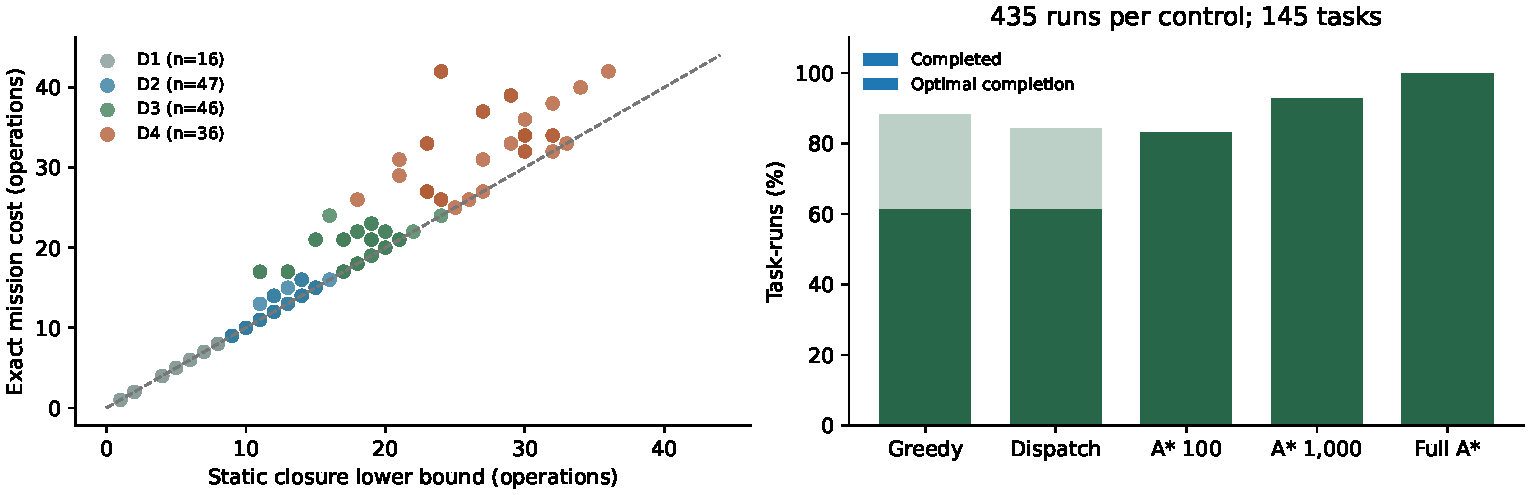
\includegraphics[width=\textwidth]{figures/mechanism-evidence.pdf}
\caption{Measured task and control evidence. Left: exact cost exceeds
the static bound on some missions; coincident points overlap. Right:
successful completion and optimal completion differ for greedy policies.
Length strata do not impose a monotonic ordering of search difficulty.
These descriptive measurements mix legacy development selection and
new-source seeded sampling, whose results should also be examined
separately.}
\label{fig:controls}
\end{figure*}

\begin{table*}[t]
\centering\small
\caption{Structural controls on 145 episodes. The oracle uses one seed;
all other policies use three tie-order seeds (435 runs). Regret is mean
excess among successful runs. Relations are privileged, so these are not
image-track VLM results.}
\begin{tabular}{lrrrrr}\toprule
Control & Runs & Success & Optimal & Regret & Max exp.\\\midrule
Exact oracle & 145 & 145 & 145 & 0.00 & ---\\
Closure greedy & 435 & 384 & 266 & 7.29 & ---\\
Capacity dispatch & 435 & 367 & 266 & 7.44 & ---\\
Closure A* (100) & 435 & 362 & 362 & 0.00 & 100\\
Closure A* (1,000) & 435 & 404 & 404 & 0.00 & 1,000\\
Closure A* (full) & 435 & 435 & 435 & 0.00 & 4,372\\
Hamming A* (full) & 435 & 435 & 435 & 0.00 & 75,454\\
Legal random & 435 & 25 & 10 & 9.76 & ---\\
Drop inspections & 435 & 156 & 156 & 0.00 & ---\\
Ignore rack limit & 435 & 239 & 239 & 0.00 & ---\\
\bottomrule\end{tabular}

\label{tab:controls}
\end{table*}

\subsection{Structural policies}
Closure greedy minimizes the static successor bound with visited-state
and randomized site tie breaking. Capacity dispatch prioritizes audits,
mandatory removals, safe placements, and temporary staging, with escape
from revisited states. Both are competent no-search controls within this
abstraction. Greedy completes 384/435 runs, dispatch 367/435, and each
achieves 266 optimal completions. Completion alone therefore conceals
substantial avoidable cost (Table~\ref{tab:controls}).

A* uses graph reopening, $(g+h,h)$ priority, and declared expansion
limits without consulting oracle tables. Caps of 100 and 1,000 expansions
complete 362 and 404 runs, respectively. Full closure A* completes all 435
optimally, with median 20 and maximum 4,372 expansions. The weaker
occupancy-plus-pending-audit heuristic also solves all runs, but uses
up to 75,454 expansions. This contrast demonstrates how a weak baseline
can inflate apparent difficulty. The full-information problem remains
computationally modest.

Dropping inspection obligations completes only 156 actual missions,
although its relaxed target is reached in every run. Ignoring the rack
limit completes 239, with 196 executor rejections. These deliberate
model-mismatch ablations diagnose omitted constraints rather than
representing strong planners. Raw actions, final states, rejection codes,
expansions, timings, and every aggregate are released. Repeated seeds
reuse source geometry, and local cached timings are not calibrated
cross-platform comparisons.

\subsection{Real model integration case}
The default explorer case runs SmolVLM-256M-Instruct on
\texttt{kart-deck-08} (public E069, seed 0). It is the first local run on
that demonstration, with all four calls retained. Each call returns a
scene description instead of a JSON action; each becomes
\texttt{INVALID\_ACTION}, consumes one operation, and leaves the physical
state unchanged. The controller then stops at the four-call limit.
This failed case verifies the actual model--feedback loop, not planning
competence or population performance.

The archive includes exact public prompts and observations, image hashes,
raw responses, parsed actions, feedback, before/after frames, latency,
measured MLX token counts, and the weight digest. Native stimuli remain
1920 pixels wide; this local model's processor resizes the longest edge
to 512 with image splitting disabled. That preprocessing is explicitly
recorded. An OpenAI-compatible vision adapter supports further practice
runs with server-side credentials. Population experiments use a separate
usage-accounted study runner.

\section{Release, limitations, and outlook}
The explorer starts with the seven task families, complete question
previews, and filters for stable ID, source, split, and length bin.
Users can attempt a question, inspect submitted-answer feedback, watch
model calls, and export review JSON. A React workbench and isolated
WebGL2 renderer retain original source geometry in live practice.
Native zoom preserves raster evidence. Dataset cards, public JSONL,
sample HD observations, evaluator dependencies, and deployment materials
are packaged together. They are local release artifacts; an external
hosting URL is not claimed.

Software validation replays all 145 optimal episodes and 739 diagnostic
answers. Additional audits check matched prefixes/action multisets,
source-group separation, repair BFS labels, budget accounting, overlapping
errors, missing assignments, and altered transcripts. Protocol and
browser tests cover persistence, idempotence, observation isolation,
question clarity, HD zoom, and model feedback. This establishes software
behavior, not human usability or hardware validity.

The principal remaining limits are empirical and structural. The public
bank is small, deterministic, and tractable with perfect relations.
Registered sites and explicit inventories simplify visual grounding.
The visual-context evidence is limited to one source and a part-count
confound. Geometry qualification omits forces, free poses, rotation,
simultaneous subassembly motion, and real rack transfers. No model
shortsightedness, human--model gap, or robustness to all shortcuts has
been measured. The next research step is the preregistered matched
image/structured study, with independent source replication and
additional count-matched geometric contrasts. BrickPlan provides
the executable instrument and falsifiable measurements for that study.

{\small
\bibliographystyle{ieeenat_fullname}
\bibliography{references}
}
\end{document}
